% Compile with: latexmk -xelatex flood_escape_article.tex
\documentclass[11pt,a4paper]{article}

\usepackage[top=2.5cm,bottom=2.5cm,left=2.6cm,right=2.6cm]{geometry}
\usepackage{amsmath,amssymb,amsthm}
\usepackage{fontspec}
\usepackage{unicode-math}
\setmainfont{Times New Roman}
\setmathfont{STIX Two Math}
\setsansfont{Arial}

\usepackage{graphicx}
\usepackage{booktabs,array,tabularx}
\usepackage{caption}
\captionsetup{font=small, labelfont=bf}
\usepackage{xcolor}
\usepackage{enumitem}
\usepackage[most]{tcolorbox}
\usepackage[hidelinks]{hyperref}

\linespread{1.1}
\hyphenation{Dijkstra}

\theoremstyle{plain}
\newtheorem{proposition}{Proposition}
\newtheorem{lemma}{Lemma}
\newtheorem{theorem}{Theorem}
\newtheorem{corollary}{Corollary}
\theoremstyle{definition}
\newtheorem{definition}{Definition}
\theoremstyle{remark}
\newtheorem{remark}{Remark}

\newcommand{\tin}{t^{\mathrm{in}}}
\newcommand{\tbl}{t^{\mathrm{bl}}}
\newcommand{\tfull}{t^{\mathrm{full}}}
\newcommand{\hb}{h_{\mathrm{b}}}
\newcommand{\vd}{v_{\mathrm{d}}}
\newcommand{\vw}{v_{\mathrm{w}}}
\newcommand{\va}{v_{\mathrm{a}}}

\begin{document}

\begin{center}
  {\LARGE\bfseries Escape Routing in Flooding Tunnel Networks:\\[4pt]
  \Large A Volume-Conserving Flood Model and Time-Dependent Shortest Paths}\\[12pt]
  {\large [Author Name]}\\[3pt]
  {\small [Affiliation]\quad$\cdot$\quad [email]}
\end{center}

\begin{abstract}
\noindent A water inrush in an underground mine changes the tunnel network on which miners must escape: tunnels become slower to walk through as they flood and impassable once the water is deep enough. We couple two models. The first is an event-driven flood model on the tunnel graph in which water spreads at a fixed front depth into level and downhill tunnels, divides equally at junctions, and backs up from dead ends. We show that the model conserves water exactly and that a network fed at a constant rate is full at the time its volume has entered, and we give its scaling with the inflow. The second is an escape-routing model in which the walking speed in a tunnel depends on its water depth at the time the miner is in it. Because the water never recedes, travel times on this time-dependent network satisfy the first-in, first-out property; consequently Dijkstra's algorithm computes earliest arrivals exactly, waiting never helps, and the latest start from which an exit can still be reached is well defined. We evaluate the models on two benchmark networks with 977 tunnels each and on a 248\,km network extracted from the plan of a working coal mine. In the benchmarks, all miners reach an exit within 20 minutes, and re-planning after a second inrush shortens escape by up to 7.6 minutes relative to the original route. In the mine network, one of 269 working faces has less than five minutes in which to start.

\medskip
\noindent\textbf{Keywords:} mine flooding; water inrush; event-driven simulation; time-dependent shortest path; FIFO property; evacuation routing
\end{abstract}

% =====================================================================
\section{Introduction}\label{sec:intro}

Water inrush is among the most serious hazards in underground coal mining: water enters suddenly through faults, boreholes or old flooded workings, and it can cut off the tunnels that lead to the shafts within minutes \cite{guo}. Deciding where each miner should go therefore requires two predictions at once: how the water will spread through the tunnel network, and how the spreading water will slow or block each possible escape route. The two are coupled through time. A tunnel that is safe now may be impassable when a miner arrives, and the best route depends on when each tunnel floods.

\paragraph{Related work.} Flow in networks of open channels and conduits is usually described by the one-dimensional Saint-Venant equations \cite{chow, cunge}, and network solvers such as the Storm Water Management Model (SWMM) \cite{swmm} integrate them on large drainage systems. Such models need hydraulic parameters --- roughness, cross-sections, boundary conditions --- that are rarely available in an emergency, and they do not by themselves produce escape routes. Routing on networks whose travel times change with time is a classical problem: Cooke and Halsey \cite{cooke} and Dreyfus \cite{dreyfus} extended shortest-path algorithms to time-dependent travel times, Kaufman and Smith \cite{kaufman} showed that label-setting algorithms remain exact when travel times satisfy the first-in, first-out (FIFO) property, and Orda and Rom \cite{orda} analysed the general case, in which waiting can be beneficial. Evacuation planning more broadly has been studied with network-flow and capacity-constrained routing models \cite{hamacher, lu}. We do not attempt a comprehensive review here.

\paragraph{This paper.} We take a deliberately simple flood model, whose rules are those of a recent modelling problem \cite{cumcm}: water advances at a fixed front depth, divides equally at junctions into level and downhill tunnels, and fills tunnels in which it cannot advance. We make this model precise, ensure that it conserves water, and couple it to an exact time-dependent routing model. Specifically:
\begin{enumerate}[leftmargin=2em, itemsep=1pt, topsep=2pt]
  \item We define an event-driven flood model for any number of inrush sources with arbitrary start times, prove that it conserves water and determine when the network is full, and bound its running time (Section~\ref{sec:flood}).
  \item We show that the travel times it induces are FIFO. Consequently, Dijkstra's algorithm is exact, waiting is never beneficial, and the latest feasible start time is well defined; this also yields a re-planning procedure for updated forecasts (Section~\ref{sec:routing}).
  \item We evaluate the models on two benchmark networks, including a delayed second inrush with re-planning, a sensitivity analysis and numerical verification (Section~\ref{sec:benchmarks}), and on a network extracted from the plan of a working coal mine (Section~\ref{sec:case}).
\end{enumerate}
Section~\ref{sec:setting} states the problem; Section~\ref{sec:discussion} discusses limitations.

% =====================================================================
\section{Problem Setting}\label{sec:setting}

\paragraph{Network.} A tunnel network is an undirected graph $G=(V,E)$. Each junction $v \in V$ has coordinates $(x_v, y_v, z_v)$, where $z_v$ is the elevation of the tunnel floor, and each tunnel $e = \{u,v\} \in E$ is the straight segment between its end junctions, of length $L_e$. All tunnels have a rectangular cross-section of width $W$ and height $H$. A point that lies inside a tunnel (an inrush location, an exit or a miner) is added to $G$ by splitting that tunnel at the point, which becomes a junction of degree two.

\paragraph{Inrush sources.} Water enters at a finite set of sources $\mathcal{S} = \{(v_j, s_j, Q_j)\}$: source $j$ discharges at constant rate $Q_j$ into junction $v_j$ from time $s_j$ onwards. The single-source case $\mathcal{S} = \{(v_1, 0, Q)\}$ is the basic scenario; a second source with $s_2 > 0$ models an inrush that occurs after the first.

\paragraph{Walking.} Miners walk at speed $\vd$ in dry tunnels. In water no deeper than $\hb$ they walk at $\vw$ in the direction of the flow and at $\va$ against it; deeper water is impassable. Miners start moving at the alert time $t_0$. A set $X \subset V$ of junctions are exits.

\paragraph{Questions.} Given $G$, $\mathcal{S}$ and the parameters of Table~\ref{tab:params}, we seek:
\begin{enumerate}[leftmargin=2em, itemsep=1pt, topsep=2pt, label=(\roman*)]
  \item a forecast of the flood: for each tunnel, when water first enters it, when it becomes impassable, and when it is full;
  \item for each miner, a route to an exit that arrives as early as possible;
  \item the latest start time from which a given route, or any route, still reaches an exit;
  \item a revised route when the forecast is updated during the escape, for example because a second source appears.
\end{enumerate}

\begin{table}[htbp]
  \centering\small
  \begin{tabular}{@{}l l l@{}}
    \toprule
    Symbol & Meaning & Value used \\
    \midrule
    $W$, $H$ & tunnel width and height & 4\,m, 3\,m \\
    $h_0$ & depth of the advancing water front & 0.1\,m \\
    $Q_j$ & inflow of source $j$ & $30\ \mathrm{m^3/min}$ \\
    $\hb$ & largest walkable depth & 0.3\,m \\
    $\vd$, $\vw$, $\va$ & walking speed: dry, with the flow, against the flow & 4, 2, 1\,m/s \\
    $t_0$ & alert time & 60\,s \\
    \midrule
    $V_e(t)$, $h_e(t)$ & stored volume and depth of tunnel $e$ & \\
    $\tin_e$, $\tbl_e$, $\tfull_e$ & times water enters $e$, $e$ becomes impassable, $e$ is full & \\
    $a_e(t)$ & time of leaving $e$ when entering it at $t$ & \\
    \bottomrule
  \end{tabular}
  \caption{Parameters and principal notation.}
  \label{tab:params}
\end{table}

% =====================================================================
\section{Flood Model}\label{sec:flood}

\subsection{Modelling assumptions}
We adopt the following idealization. Water advances along a tunnel as a front of constant depth $h_0$, so that covering tunnel $e$ requires the volume $W h_0 L_e$. At a junction, water divides equally among the tunnels into which it can flow, preferring level and downhill tunnels. Water accumulates only where it cannot advance; the water surface in a tunnel is taken to be level along the tunnel, so that its depth is $h_e = V_e/(W L_e)$.

\begin{remark}[Why conservation must be imposed]\label{rem:naive}
A natural event-driven implementation lets a tunnel that has just been covered start to fill at its inflow $q$ while passing the same $q$ on to the next tunnels. Already for two tunnels in series, the network then stores water at rate $2q$ while only $q$ enters. On the benchmark network N1 of Section~\ref{sec:benchmarks}, such a scheme predicts a median arrival time of 445 days at the junctions and leaves some junctions dry for about 16{,}000 years, whereas the conserving model below fills the whole network in 35 days. A second common simplification, forbidding flow into uphill tunnels altogether, leaves 635 of the 663 junctions of the three-dimensional network N2 dry forever. The model below avoids both problems.
\end{remark}

\subsection{State and rules}

\begin{definition}[State]
At time $t$, every tunnel $e$ has a stored volume $V_e(t) \in [0, WHL_e]$ and a mode
\[
  \mu_e(t) \in \{\textsf{dry}, \textsf{covering}, \textsf{conveying}, \textsf{storing}, \textsf{full}\}.
\]
A \textsf{covering} tunnel is being covered by a front of depth $h_0$; a \textsf{conveying} tunnel passes its entire inflow to its far end without storing more; a \textsf{storing} tunnel accumulates its inflow. A junction is \emph{wet} from the time water first reaches it, and every wet junction that is not a source has a \emph{feeding tunnel} $\pi(v)$: the conveying tunnel through which water first reached it.
\end{definition}

For a wet junction $v$ let $C(v)$ be the set of tunnels at $v$ that are not full, excluding $\pi(v)$ while it is conveying, and let $D(v) \subseteq C(v)$ contain the tunnels whose other end is not higher than $v$. The \emph{outlets} of $v$ are $O(v) = D(v)$ if $D(v) \neq \emptyset$ and $O(v) = C(v)$ otherwise.

\begin{definition}[Flow rules]\label{def:rules}
At every time, flows are determined as follows.
\begin{enumerate}[leftmargin=2.2em, itemsep=2pt, topsep=2pt, label=\textbf{R\arabic*}]
  \item \emph{(Division.)} The inflow $\phi_v$ of a wet junction $v$ is the sum of the discharges of active sources at $v$ and the flow conveyed by $\pi(v)$. It is divided equally among $O(v)$. A dry outlet becomes \textsf{covering} if it is level or downhill from $v$; otherwise it becomes \textsf{storing} and fills from its lower end.
  \item \emph{(Covering.)} When $V_e$ reaches $W h_0 L_e$, a covering tunnel fed from one end $u$ only becomes \textsf{conveying} if its far end $w$ is dry; $w$ becomes wet with $\pi(w) = e$. Otherwise it becomes \textsf{storing}.
  \item \emph{(Backing up.)} If $\phi_v > 0$ and $O(v) = \emptyset$, the feeding tunnel $\pi(v)$ stops conveying: it becomes \textsf{storing} if it is not full, and \textsf{full} otherwise. If $v$ is a source and has no feeding tunnel that can store water, its discharge is transferred, through full tunnels, to the nearest junction (by tunnel length) that has an outlet or a feeding tunnel that can still store water.
  \item \emph{(Overtopping.)} When $V_e$ reaches $WHL_e$, $e$ becomes \textsf{full}. If $e$ was entered from its lower end and its upper end $w$ is dry, it instead becomes \textsf{conveying}, $w$ becomes wet and $\pi(w) = e$.
\end{enumerate}
For each tunnel we record $\tin_e$, the first time it receives water; $\tbl_e$, the first time $h_e(t) > \hb$; and $\tfull_e$, the time it becomes full.
\end{definition}

Rule R1 is the division rule of the problem setting. R2--R4 specify what happens when water cannot advance: it is stored in the tunnel that delivered it, and the storage moves upstream as tunnels fill. Because each junction acquires its feeding tunnel when it first becomes wet, from a junction that was wet earlier, the feeding tunnels form a forest rooted at the sources, and every junction can be processed after its feeding tunnel.

\subsection{Event-driven simulation}

Between consecutive events all modes, and therefore all flows, are constant, so every stored volume grows linearly. An event occurs when a tunnel's volume reaches $W h_0 L_e$ (covered), $\hb W L_e$ (impassable) or $W H L_e$ (full), or when a source starts. Algorithm~1 advances from event to event.

\begin{tcolorbox}[colback=white, colframe=black!60, boxrule=0.5pt, arc=0pt, left=6pt, right=6pt, top=4pt, bottom=4pt, fontupper=\small,
  title={\small\textbf{Algorithm 1.} Event-driven flood simulation}, coltitle=black, colbacktitle=black!8]
\textbf{Input:} graph $G$, sources $\mathcal{S}$, parameters $W, H, h_0, \hb$.\quad \textbf{Output:} $\tin_e, \tbl_e, \tfull_e$ for all $e \in E$.
\begin{enumerate}[label=\arabic*:, leftmargin=1.8em, itemsep=1pt, topsep=3pt]
  \item $t \gets 0$; all tunnels \textsf{dry} with $V_e = 0$; activate the sources with $s_j = 0$.
  \item \textbf{repeat}
  \item \quad\emph{Distribute:} visit the wet junctions in the order in which they became wet; compute $\phi_v$, apply R1 and, where $O(v) = \emptyset$, R3. If R3 changes the mode of a tunnel that has already received flow in this pass, restart the pass.
  \item \quad\emph{Next event:} $\Delta \gets$ the least time until a receiving tunnel reaches its next threshold volume or the next source starts.
  \item \quad\emph{Advance:} $t \gets t + \Delta$; $V_e \gets V_e + \Delta \cdot (\text{inflow of } e)$ for all $e$; record $\tbl_e$ and $\tfull_e$ where reached.
  \item \quad\emph{Transitions:} apply R2 and R4; activate sources with $s_j = t$.
  \item \textbf{until} no tunnel receives water and no source is pending.
\end{enumerate}
\end{tcolorbox}

\begin{proposition}[Running time]\label{prop:time}
Algorithm~1 performs at most $3|E| + |\mathcal{S}|$ events and runs in $O\bigl((|E| + |\mathcal{S}|)(|V| + |E|)\bigr)$ time.
\end{proposition}
\begin{proof}
Each tunnel reaches each of its three threshold volumes at most once, and each source starts once. A distribution pass takes $O(|V| + |E|)$ time. A pass is restarted only when a tunnel changes mode irreversibly (at most a bounded number of times per tunnel) or when a source's discharge is transferred (at most once per source and event), which adds $O(|E| + |\mathcal{S}|)$ passes in total.
\end{proof}

In our implementation (Python), simulating a 977-tunnel network until it is full takes about one second.

\subsection{Properties}

\begin{proposition}[Conservation and filling time]\label{prop:conservation}
Let $G$ be connected with total volume $\mathcal{V} = \sum_{e} W H L_e$. As long as some tunnel is not full, the volume stored at time $t$ equals the volume that has entered,
\begin{equation}
  \sum_{e\in E} V_e(t) = \sum_{j} Q_j\,(t - s_j)^+ .
  \label{eq:conservation}
\end{equation}
Consequently the last tunnel becomes full at the unique $t^*$ with $\sum_j Q_j (t^* - s_j)^+ = \mathcal{V}$; for a single source starting at $0$, $t^* = \mathcal{V}/Q$.
\end{proposition}
\begin{proof}
Under R1 every junction passes its entire inflow to its outlets; a conveying tunnel passes its inflow on, and covering and storing tunnels store it. Flow is therefore neither created nor lost unless some junction $v$ has $\phi_v > 0$ and $O(v) = \emptyset$. In that case R3 either turns $\pi(v)$ into a storing tunnel, which absorbs the flow, or, if $v$ is a source whose surrounding tunnels are all full, transfers the discharge through full tunnels to a junction that can absorb it. Such a junction exists whenever some tunnel is not full, because $G$ is connected and the tunnels adjacent to wet junctions are either full or able to receive water. Hence the total storage rate equals the total discharge at all times before $t^*$, which proves \eqref{eq:conservation}. The left-hand side cannot exceed $\mathcal{V}$, so all tunnels are full at $t^*$; and since the right-hand side increases strictly after the first source starts, no earlier time has this property.
\end{proof}

\begin{proposition}[Scaling with the inflow]\label{prop:scaling}
If all sources start at time $0$ and every $Q_j$ is multiplied by $\lambda > 0$, then every time recorded by Algorithm~1 is multiplied by $1/\lambda$.
\end{proposition}
\begin{proof}
Flows are the discharges multiplied by fractions that depend only on $G$ and on the modes, and each event occurs when a volume determined by $G$ is reached. Suppose the two runs have processed the same events, with the times of the scaled run equal to $1/\lambda$ times the original ones. Then both runs are in the same state, with all flows multiplied by $\lambda$, so the next event is the same and its time is likewise multiplied by $1/\lambda$. Induction over events completes the proof.
\end{proof}

The proposition fails when a source starts at a fixed positive time, since that start time does not scale.

\begin{proposition}[Attenuation of the front]\label{prop:attenuation}
Let a front leave a source along tunnels $e_1, \dots, e_k$, before any tunnel stores water. Let $m_0$ be the number of outlets at the source and $m_i$ the number of outlets at the far end of $e_i$. Then $e_k$ receives the flow $q_k = Q/(m_0 m_1 \cdots m_{k-1})$ and is covered in time $W h_0 L_{e_k} / q_k$.
\end{proposition}
\begin{proof}
By R1 the flow is divided by $m_i$ at each junction, and a covering tunnel of length $L$ fed at rate $q$ is covered after $W h_0 L / q$.
\end{proof}

In networks where most junctions have degree three, $m_i = 2$ and the time needed to cover a tunnel doubles at each junction: the front decelerates geometrically. Proposition~\ref{prop:conservation} shows that this deceleration does not delay filling indefinitely, because water that cannot advance is stored and, as tunnels fill, redistributed to the remaining ones.

% =====================================================================
\section{Escape Routing}\label{sec:routing}

\subsection{Travel time through a tunnel}
The flood forecast assigns to each tunnel the times $\tin_e$ and $\tbl_e$ and a flow direction, given by the end from which it first received water. The walking speed in $e$ at time $t$ is
\begin{equation}
  \sigma_e(t) = \begin{cases}
    \vd, & t < \tin_e,\\
    u_e, & \tin_e \le t \le \tbl_e,\\
    0, & t > \tbl_e,
  \end{cases}
  \label{eq:speed}
\end{equation}
where $u_e = \vw$ or $\va$ according to the walking direction relative to the flow. Treating the whole tunnel as wet from $\tin_e$ is conservative, because the front is still advancing during $[\tin_e, \tin_e + W h_0 L_e/q]$. Since $\sigma_e$ changes at most twice, the time at which a miner entering $e$ at time $t$ leaves it is
\begin{equation}
  a_e(t) = \begin{cases}
    t + L_e/\vd, & L_e \le \vd\,(\tin_e - t)^+,\\[3pt]
    \max(t, \tin_e) + \dfrac{L_e - \vd\,(\tin_e - t)^+}{u_e}, & \text{otherwise},
  \end{cases}
  \label{eq:arrival}
\end{equation}
with $a_e(t) = \infty$ if the right-hand side exceeds $\tbl_e$. Evaluating \eqref{eq:arrival} exactly matters: discretizing the tunnel into segments with constant speed can misclassify feasibility near $\tbl_e$. For example, a 20\,m tunnel that becomes wet at 4.1\,s ($u_e = 2$\,m/s) is left at 5.9\,s, whereas 20 equal segments evaluated at their entry times give 5.75\,s; if the tunnel becomes impassable at 5.77\,s, the discretized model wrongly admits it.

A \emph{route} is a sequence of tunnels $P = (e_1, \dots, e_m)$ joined end to end from the miner's position to an exit; starting at $t$, the miner reaches the exit at $A_P(t) = a_{e_m}(\cdots a_{e_1}(t))$.

\subsection{The FIFO property and exact routing}

\begin{lemma}[FIFO]\label{lem:fifo}
For every tunnel $e$ and walking direction, $a_e$ is non-decreasing.
\end{lemma}
\begin{proof}
By \eqref{eq:speed} the speed in $e$ depends only on time, not on position, and is non-increasing in time. Let two miners enter $e$ at times $t_1 \le t_2$. At time $t_2$ the first miner is ahead of the second or has left the tunnel; thereafter both move with the same speed, so the distance between them does not decrease and the first leaves no later than the second. If the tunnel becomes impassable before the first miner leaves, it does so before the second leaves as well, and $a_e(t_1) = a_e(t_2) = \infty$.
\end{proof}

\begin{theorem}\label{thm:dijkstra}
Consider Dijkstra's algorithm \cite{dijkstra} started from the miner's position $r$ with label $\tau(r) = t_0$, in which settling junction $u$ updates every neighbour $w$ by $\tau(w) \gets \min\{\tau(w), a_{uw}(\tau(u))\}$. When a junction is settled, its label equals the earliest time at which it can be reached from $r$ departing at $t_0$. Moreover, waiting at a junction never yields an earlier arrival.
\end{theorem}
\begin{proof}
The second claim follows from Lemma~\ref{lem:fifo}: departing from $u$ at $t' \ge t$ gives $a_{uw}(t') \ge a_{uw}(t)$. For the first, suppose that all junctions settled so far carry correct labels, that $u$ is the next junction to be settled, and that some route reaches $u$ at time $T < \tau(u)$. Let $(x, y)$ be the first tunnel of this route that leaves the settled set. The route reaches $x$ no earlier than $\tau(x)$, so by Lemma~\ref{lem:fifo} it reaches $y$ no earlier than $a_{xy}(\tau(x))$, a value already used to update $\tau(y)$. Since $a_e(t) \ge t$ for all $e$, arrival times along the route do not decrease, so $\tau(y) \le T < \tau(u)$. The algorithm would then have settled $y$ before $u$, a contradiction.
\end{proof}

Stopping the search at the first exit settled yields the earliest-arriving route and its exit. These results are instances of the general theory of FIFO networks \cite{kaufman, orda}; the point here is that the FIFO property follows from the flood model, because water levels never decrease.

\begin{corollary}[Latest start]\label{cor:latest}
For a fixed route $P$, the set of start times from which $P$ reaches its exit is an interval $(-\infty, D(P)]$. Likewise, the set of start times from which some exit can be reached is an interval $(-\infty, D^*]$.
\end{corollary}
\begin{proof}
$A_P$ is a composition of non-decreasing functions and is therefore non-decreasing, so if $A_P(t) < \infty$ then $A_P(t') \le A_P(t) < \infty$ for all $t' \le t$. The second statement follows by taking the union over routes.
\end{proof}

For a fixed route, $D(P)$ is obtained exactly by inverting \eqref{eq:arrival} tunnel by tunnel from the exit backwards. If $d$ is the latest admissible exit time of $e$, the latest admissible entry time is
\[
  b_e(d) = \begin{cases}
    z - L_e/u_e, & L_e \le u_e\,(z - \tin_e)^+,\\
    \min(z, \tin_e) - \bigl(L_e - u_e\,(z - \tin_e)^+\bigr)/\vd, & \text{otherwise},
  \end{cases}
  \qquad z = \min(d, \tbl_e),
\]
and $D(P) = b_{e_1}(\cdots b_{e_m}(\infty))$. By Corollary~\ref{cor:latest}, $D^*$ can be found by bisection on the start time, using Theorem~\ref{thm:dijkstra} to test feasibility. The quantity $D^*$ is the latest alert that still leaves the miner a way out.

\subsection{Re-planning under an updated forecast}\label{sec:replan}
Suppose the forecast is replaced at time $\tau$, for instance because a second source starts at $s_2 < \tau$. A miner who has followed route $P$ from $t_0$ is then at some point of a tunnel $(a, b)$, at distance $\xi$ from $a$, obtained by evaluating \eqref{eq:arrival} along $P$. We add a junction $r$ at this point, connected to $a$ and $b$ by tunnels of lengths $\xi$ and $L_{ab} - \xi$ that inherit $\tin_{ab}$, $\tbl_{ab}$ and the flow direction of $(a, b)$ under the new forecast, and run the search of Theorem~\ref{thm:dijkstra} from $r$ with label $\tau$. The miner may thus continue or turn back. We compare the result with the time obtained by continuing along the remainder of $P$ under the new forecast.

% =====================================================================
\section{Benchmark Networks}\label{sec:benchmarks}

\subsection{Setup}
The two benchmark networks of \cite{cumcm}, which we denote N1 and N2, have the same topology: 663 junctions, 977 tunnels and a total length of 125.6\,km; 501 of the junctions (76\%) have degree three. N1 is planar ($z = 10$\,m throughout); N2 is three-dimensional, with elevations between 0 and 71.5\,m (Figure~\ref{fig:networks}). Each network has a primary source A starting at $t=0$, a secondary source B starting 240\,s (N1) or 300\,s (N2) later, two exits E1 and E2 and three miners M1--M3; their coordinates are listed in Appendix~\ref{app:coords}. All given points lie on the network to within 0.016\,m and are inserted into the graph as described in Section~\ref{sec:setting}. Parameters are those of Table~\ref{tab:params}.

\begin{figure}[htbp]
  \centering
  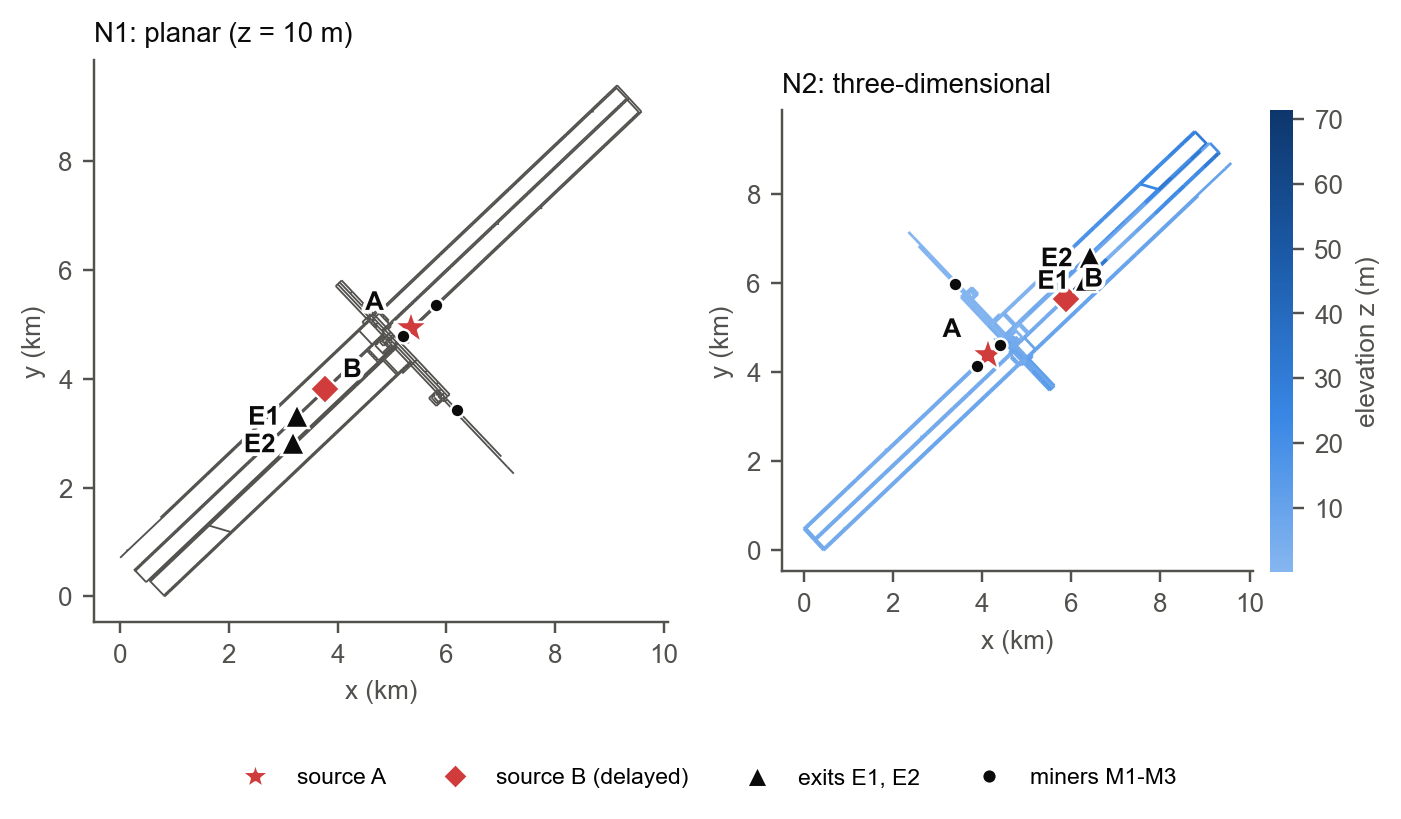
\includegraphics[width=\textwidth]{figures/networks.png}
  \caption{The benchmark networks N1 (planar) and N2 (three-dimensional, coloured by elevation), with sources, exits and miners.}
  \label{fig:networks}
\end{figure}

\subsection{Flood propagation}
Figure~\ref{fig:arrival} shows the time at which water first enters each tunnel, and Table~\ref{tab:flood} summarizes the time scales. With a single source, water spreads along the main roadways of N1 in both directions; in N2 it first runs downhill towards the south-west and reaches higher tunnels only when no level or downhill outlet remains. Both networks are full after 34.9 days, in agreement with Proposition~\ref{prop:conservation} ($\mathcal{V}/Q = 837.0$\,h for N1 and 837.5\,h for N2). With the delayed second source, the median arrival time at the junctions decreases by 61\% (N1) and 39\% (N2), and the networks are full after $t^* = \mathcal{V}/(2Q) + s_2/2$, again as Proposition~\ref{prop:conservation} predicts.

\begin{figure}[htbp]
  \centering
  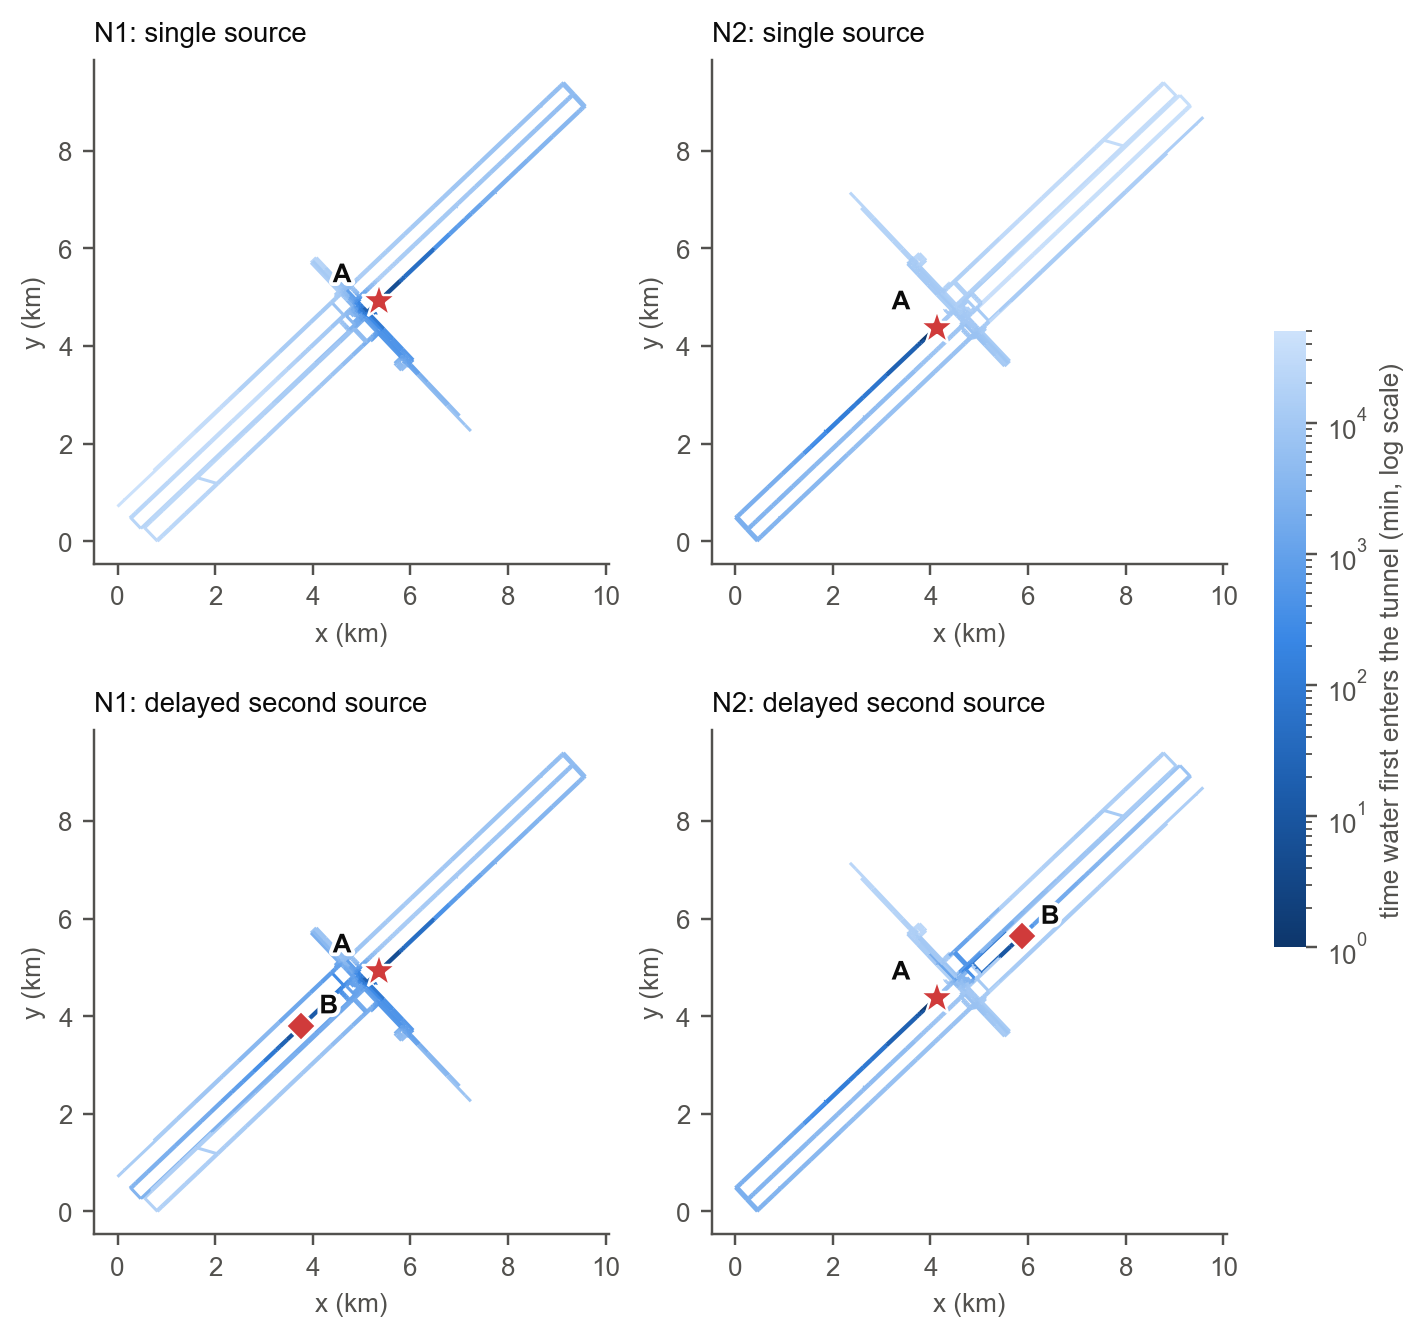
\includegraphics[width=0.9\textwidth]{figures/arrival_maps.png}
  \caption{Time at which water first enters each tunnel, for a single source (top) and with the delayed second source (bottom).}
  \label{fig:arrival}
\end{figure}

\begin{table}[htbp]
  \centering\small
  \begin{tabular}{@{}l l c c c@{}}
    \toprule
    Network & Sources & Median arrival at a junction & Last junction reached & Network full \\
    \midrule
    N1 & A        & 4.4 d & 31.9 d & 34.9 d \\
    N1 & A and B  & 1.7 d & 13.8 d & 17.4 d \\
    N2 & A        & 8.2 d & 29.1 d & 34.9 d \\
    N2 & A and B  & 5.0 d & 17.1 d & 17.4 d \\
    \bottomrule
  \end{tabular}
  \caption{Flood time scales on the benchmark networks. In every case all junctions and tunnels are eventually reached and filled.}
  \label{tab:flood}
\end{table}

\subsection{Escape routes}
Table~\ref{tab:routes} and Figure~\ref{fig:routes} give the earliest-arriving routes for the single-source forecast. For comparison, we also evaluate the shortest route by length --- the route a miner would choose ignoring the flood --- under the same forecast.

\begin{table}[htbp]
  \centering\small
  \begin{tabular}{@{}c c c c c c c@{}}
    \toprule
    Network & Miner & Exit & Arrival & Length & Latest start & Shortest route \\
            &       &      & (min)   & (km)   & $D(P)$       & by length (min) \\
    \midrule
    N1 & M1 & E1 & 15.9 & 3.57 & 26.6 min & 19.3 \\
    N1 & M2 & E1 & 12.2 & 2.68 & 7.8 h    & identical \\
    N1 & M3 & E1 & 18.1 & 4.10 & 26.8 h   & identical \\
    N2 & M1 & E1 & 12.2 & 2.69 & 7.0 d    & identical \\
    N2 & M2 & E1 & 18.1 & 4.11 & 8.6 d    & identical \\
    N2 & M3 & E1 & 19.2 & 3.44 & 21.5 h   & 19.7 \\
    \bottomrule
  \end{tabular}
  \caption{Earliest-arriving routes for a single source and $t_0 = 1$\,min. Times are measured from the onset of the inrush.}
  \label{tab:routes}
\end{table}

\begin{figure}[htbp]
  \centering
  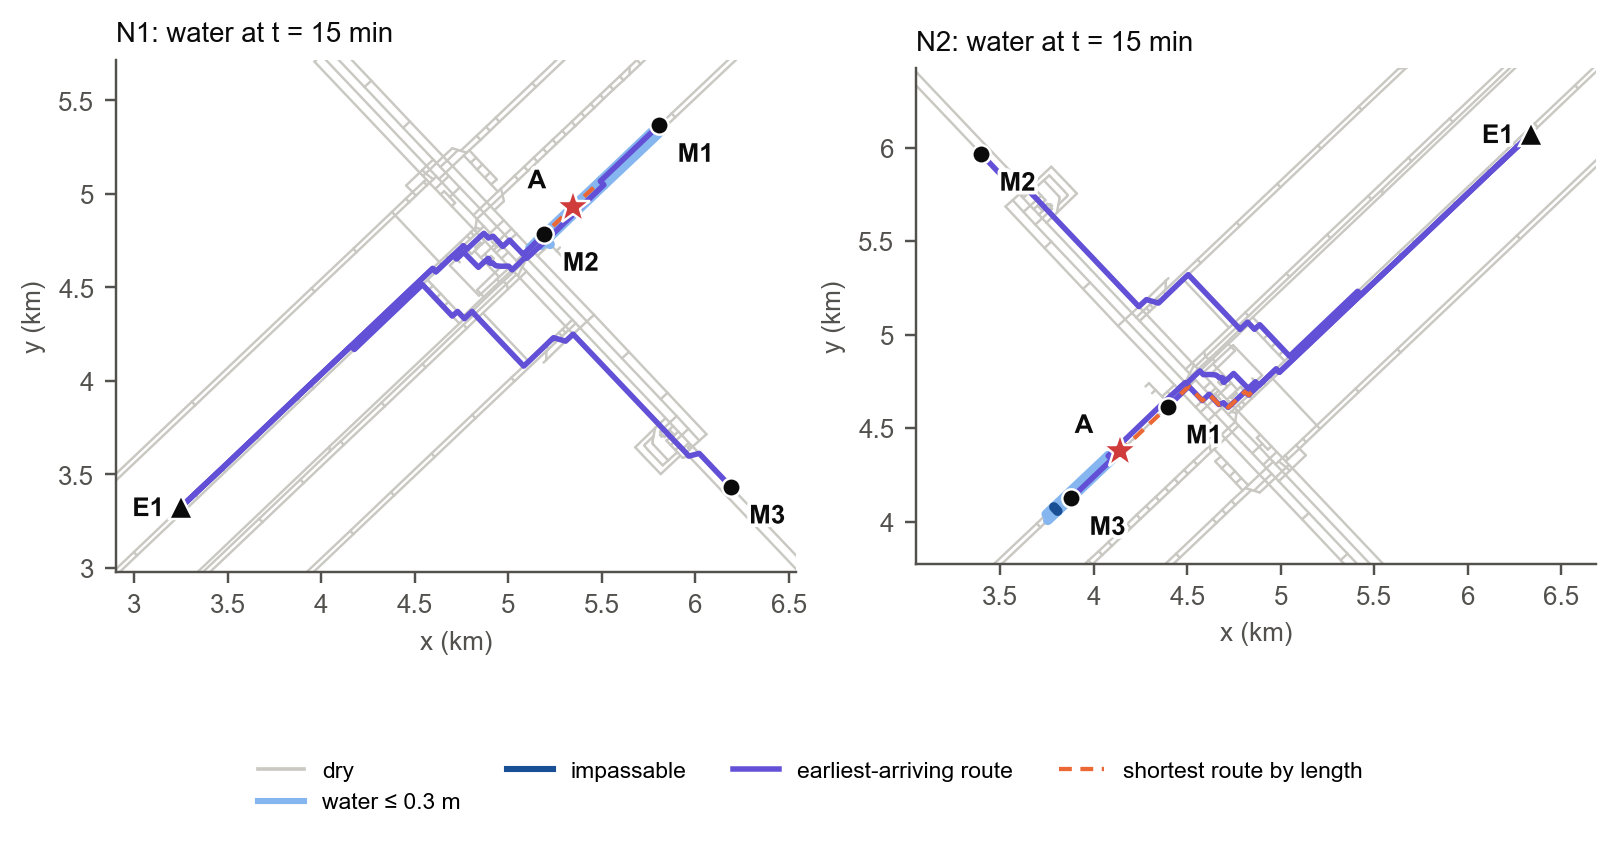
\includegraphics[width=\textwidth]{figures/routes_single.png}
  \caption{Earliest-arriving routes and the flood 15\,min after the onset, single source. Where the shortest route by length differs, it is shown dashed.}
  \label{fig:routes}
\end{figure}

All six miners reach exit E1 between 12 and 20 minutes after the onset. Five of the routes remain dry throughout, so the miners walk at $\vd$ the entire way. For four miners the earliest-arriving route coincides with the shortest route by length, because the water does not reach that route in time. In N1, M1 starts close to the source: the shortest route passes through tunnels that are already wet and arrives at 19.3\,min, whereas a route 40\,m longer remains dry and arrives at 15.9\,min. This route has the smallest margin in the table, since it must be started by $D(P) = 26.6$\,min. In N2, M3 starts 0.36\,km from the source and slightly below it, and every route out passes through wet tunnels; the earliest-arriving route still improves on the shortest route by 0.5\,min.

\subsection{A delayed second source and re-planning}
Source B starts at $s_2 = 240$\,s (N1) or 300\,s (N2), and the revised plan is issued at $\tau = s_2 + 60$\,s, following Section~\ref{sec:replan}. At $\tau$ every miner is inside a tunnel. Positions computed by walking the original routes through the updated flood coincide with those under the original forecast, so the water from B does not affect the part of any route walked before $\tau$. Table~\ref{tab:replan} and Figure~\ref{fig:replan} compare the revised routes with continuing along the original ones.

\begin{table}[htbp]
  \centering\small
  \begin{tabular}{@{}c c c c c c@{}}
    \toprule
    Network & Miner & Exit & \multicolumn{2}{c}{Arrival (min)} & Latest start \\
    \cmidrule(lr){4-5}
            &       & (revised) & revised route & original route & of revised route \\
    \midrule
    N1, $\tau = 5$ min & M1 & E2 & 16.5 & 20.7 & 95 min \\
                       & M2 & E1 & 15.2 & 17.0 & 24.2 min \\
                       & M3 & E2 & 18.5 & 26.1 & 56 h \\
    \midrule
    N2, $\tau = 6$ min & M1 & E1 & 12.4 & 16.3 & 9.1 min \\
                       & M2 & E2 & 18.5 & 26.0 & 80 min \\
                       & M3 & E2 & 19.8 & 27.1 & 79 min \\
    \bottomrule
  \end{tabular}
  \caption{Re-planning at time $\tau$ after the second source starts. Times are measured from the onset of the first inrush.}
  \label{tab:replan}
\end{table}

\begin{figure}[htbp]
  \centering
  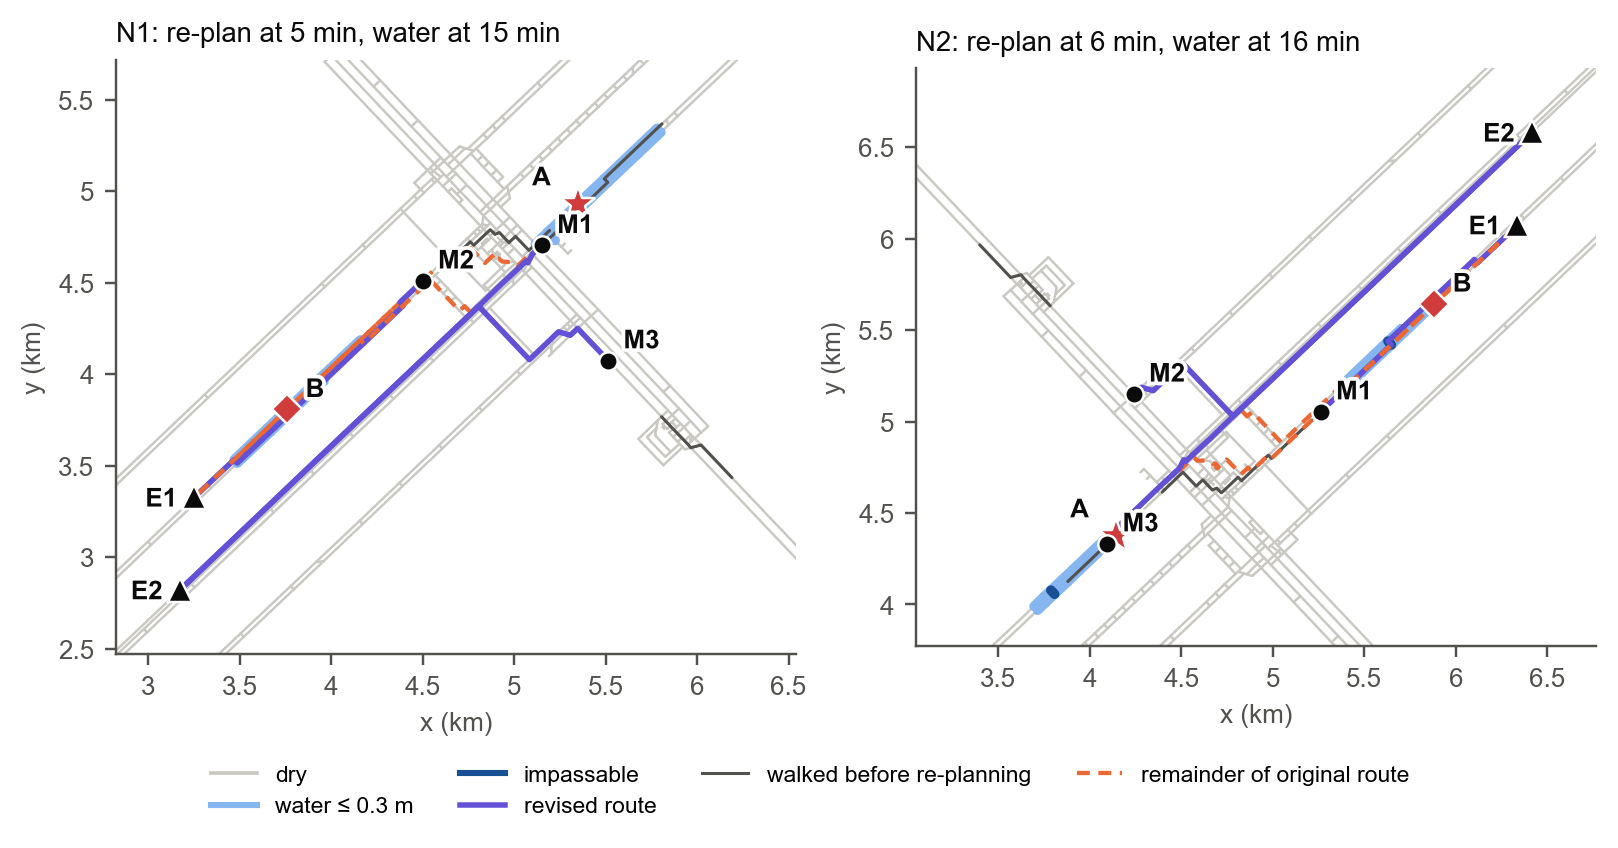
\includegraphics[width=\textwidth]{figures/routes_replan.png}
  \caption{Re-planning after the second source starts. Grey: the part of the original route walked before $\tau$; dashed: the remainder of the original route; solid: the revised route. The flood is shown 10\,min after $\tau$.}
  \label{fig:replan}
\end{figure}

All six revised routes differ from the original routes, and four of them lead to the other exit: in both networks B lies 0.6--0.7\,km from E1, close to the original routes. Continuing along the original routes would not trap any miner, but it would delay arrival by 1.7--7.6 minutes, because those routes cross water from B. Compared with the single-source plans, the second source delays the earliest arrival by 0.2--3.1 minutes. The smallest margin occurs in N2 for M1, whose revised route must be started by 9.1 minutes; a revised plan issued three minutes later than assumed would no longer make that route feasible.

\subsection{Sensitivity}
We varied one parameter at a time and recomputed the flood and the six routes for the single-source scenario (Table~\ref{tab:sens}). Changing the inflow or the front depth by $\pm10\%$ leaves all six arrival times and routes unchanged. By Proposition~\ref{prop:scaling}, a 10\% larger inflow shortens every flood time by 9.1\%, but the walking speed in every tunnel along the routes is unaffected. The walking speeds in water affect only the routes that pass through water. The alert time has the largest effect. A later alert can force a longer route: with an alert after 10 minutes, the walking time of M1 in N1 increases by 48\%. With an alert at the onset, the walking time of M3 in N2 decreases by 14\% on the same route, because some of its tunnels are then entered before they are wet.

\begin{table}[htbp]
  \centering\small
  \begin{tabular}{@{}l c c c c@{}}
    \toprule
    Parameter & Change & Mean change of walking time & Largest change & Routes changed \\
    \midrule
    Inflow $Q$                & $\pm10\%$ & 0 & 0 & 0 of 6 \\
    Front depth $h_0$         & $\pm10\%$ & 0 & 0 & 0 of 6 \\
    Speed with the flow $\vw$ & $+10\%$ / $-10\%$ & $-0.02\%$ / $+0.02\%$ & 0.14\% & 0 of 6 \\
    Speed against the flow $\va$ & $+10\%$ / $-10\%$ & $-0.4\%$ / $+0.5\%$ & 3.0\% & 0 of 6 \\
    Alert time $t_0$          & 0 min  & $-2.4\%$ & 14\% & 0 of 6 \\
                              & 2 min  & 0        & 0    & 0 of 6 \\
                              & 5 min  & $+2.8\%$ & 17\% & 1 of 6 \\
                              & 10 min & $+8.4\%$ & 48\% & 1 of 6 \\
                              & 20 min & $+8.7\%$ & 48\% & 1 of 6 \\
    \bottomrule
  \end{tabular}
  \caption{Sensitivity of the six routes of Table~\ref{tab:routes}. Walking time is arrival time minus $t_0$; the baseline is $t_0 = 1$\,min.}
  \label{tab:sens}
\end{table}

\subsection{Numerical verification}
\begin{itemize}[leftmargin=1.5em, itemsep=2pt, topsep=2pt]
  \item \emph{Conservation.} After every event, \eqref{eq:conservation} holds to a relative error below $4\times10^{-15}$, and the last tunnel becomes full at $\mathcal{V}/Q$ to twelve significant digits.
  \item \emph{Scaling.} With inflow $1.1\,Q$, each of the approximately 3{,}900 recorded times per network equals $1/1.1$ times its original value to thirteen significant digits (Proposition~\ref{prop:scaling}).
  \item \emph{Routing.} On 150 random graphs with seven junctions and random wetting and blocking times, the arrival time of Theorem~\ref{thm:dijkstra} equals the minimum over all simple routes. On 2{,}000 random tunnels, $a_e$ is non-decreasing and $b_e$ inverts it.
  \item \emph{Discretization.} Splitting tunnels changes the sequence of events, so the forecast depends on how the network is discretized. We inserted ten degree-two junctions at random positions in 20 independent trials per network. Of the resulting junction arrival times, 80\% (N1) and 89\% (N2) are unchanged, and 95\% change by less than 0.21\% (N1) and 0.004\% (N2). The 99th percentiles are 5.5\% and 0.4\%; the largest relative changes, 41\% and 31\%, are local and arise where a split changes the outcome of rule R2 or the order in which tunnels back up.
\end{itemize}

% =====================================================================
\section{Case Study: A Working Coal Mine}\label{sec:case}

\subsection{Network extraction}
We applied the method to the mining plan of a working longwall coal mine, an AutoCAD drawing at scale 1:10{,}000 with 87 layers. The plan was read with LibreDWG \cite{libredwg}, and the network was built as follows.
\begin{enumerate}[leftmargin=2em, itemsep=1pt, topsep=2pt]
  \item \emph{Tunnels} were taken from the centerline layer (576 polylines). Gaps of less than 8\,m between the end of one centerline and another centerline --- typically a crosscut ending just short of a roadway --- were bridged (605 gaps); all lines were then split at their intersections, and the largest connected component was retained.
  \item \emph{Elevations} were obtained from the 2{,}347 survey stations annotated with the measured roof elevation; each junction received the inverse-distance-weighted mean of the stations within 300\,m.
  \item \emph{Width.} The median distance between the two drawn walls of a roadway is $W = 5.0$\,m; the height is not recorded on the plan, and we used $H = 3$\,m.
  \item \emph{Exits} are the bottoms of the four shafts, each joined to the nearest junction (connections of 10--66\,m).
\end{enumerate}
The resulting network has 1{,}591 junctions, 2{,}083 tunnels and 248\,km of roadway, with a median gradient of 0.9\%. Coordinates were rotated, reflected and translated, and elevations are given relative to an arbitrary datum (Figure~\ref{fig:mine}).

\begin{figure}[htbp]
  \centering
  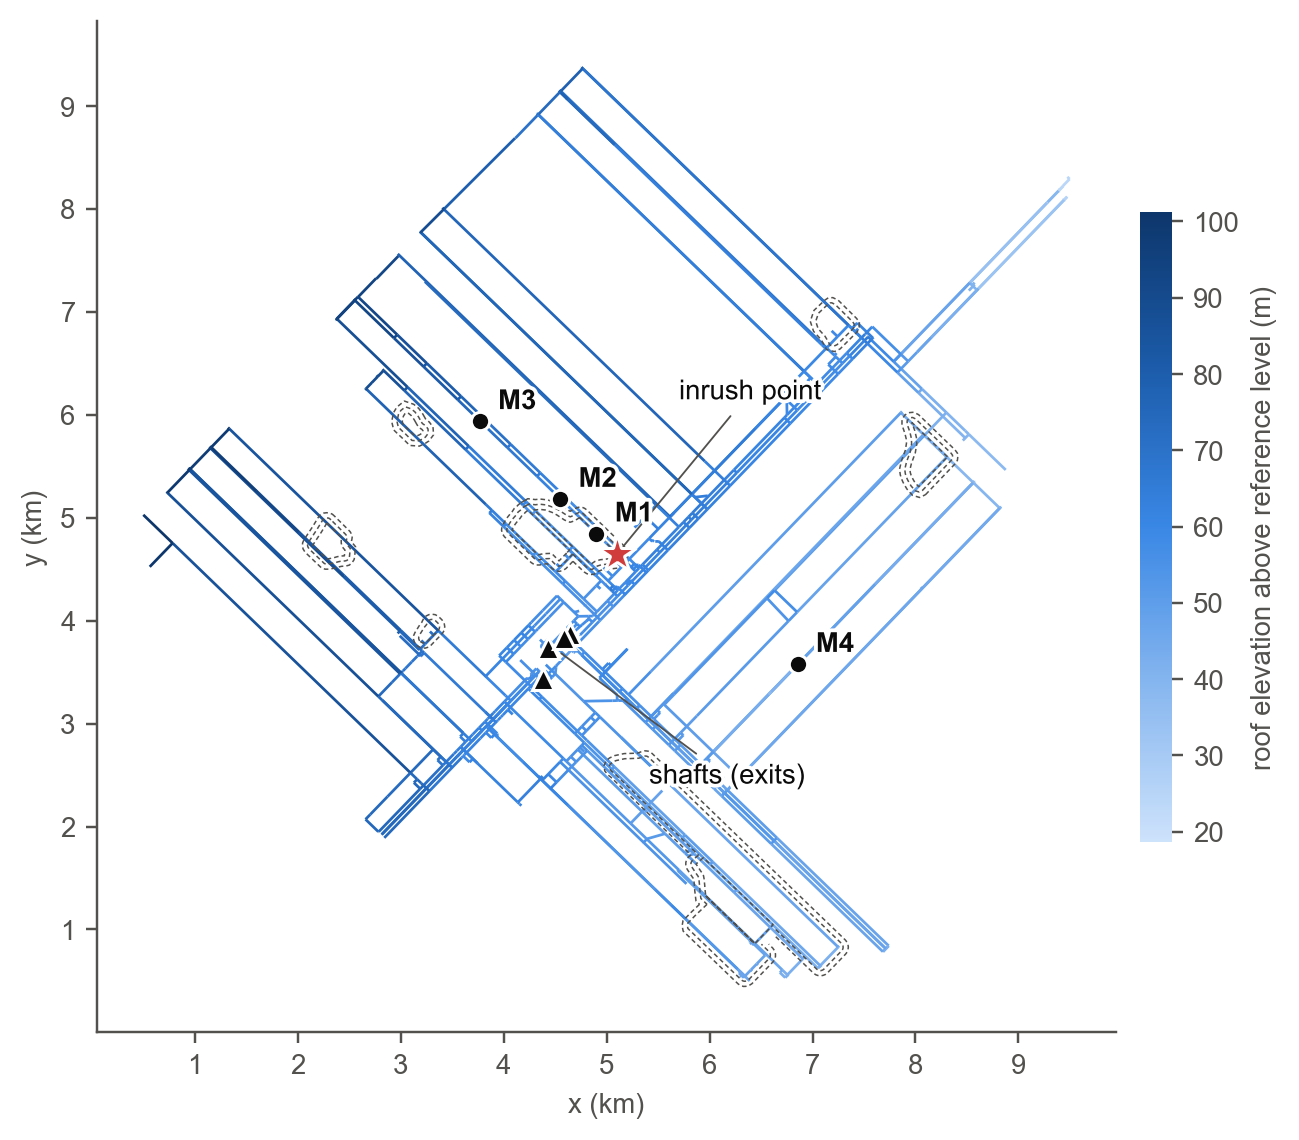
\includegraphics[width=0.74\textwidth]{figures/mine_network.png}
  \caption{Network extracted from the plan of a working coal mine, coloured by roof elevation relative to an arbitrary datum. Dashed outlines mark the zones of accumulated water recorded on the plan.}
  \label{fig:mine}
\end{figure}

\subsection{Scenario}
The plan records several zones of water accumulated in old workings. We let the zone closest to the shafts (by tunnel distance) discharge into the roadway it touches, at $Q = 30\ \mathrm{m^3/min}$; all other parameters are as in Table~\ref{tab:params}, with $W = 5.0$\,m. The source lies 1.2\,km from the nearest shaft. We evaluate every working face, defined as a dead end of the network (269 faces), and report four representative faces in detail: three faces 0.3, 0.8 and 1.9\,km from the source whose routes out pass near it (M1--M3), and one face 4.3\,km away on the far side of the mine (M4).

\subsection{Results}
The flood remains local for hours: after one hour 1.7\,km of the 248\,km of roadway are wet and 0.5\,km impassable, and after one day 4.4\,km and 3.3\,km. The median arrival time at a junction is 18.1 days, and the network is full after 85.9 days, equal to $\mathcal{V}/Q$.

Across all 269 faces, with an alert after one minute, the shortest route by length remains passable from every face. It is also the earliest-arriving route from 261 faces; from the remaining 8 faces, accounting for the flood shortens the escape by up to 9.6 minutes. The latest alert $D^*$ has a median of 13.1 days; it is below one day for 5 faces and below one hour for one face, where it is 4 minutes 40 seconds. Table~\ref{tab:mine} gives the four representative faces, and Table~\ref{tab:mine-alert} shows the effect of the alert time.

\begin{figure}[!htb]
  \centering
  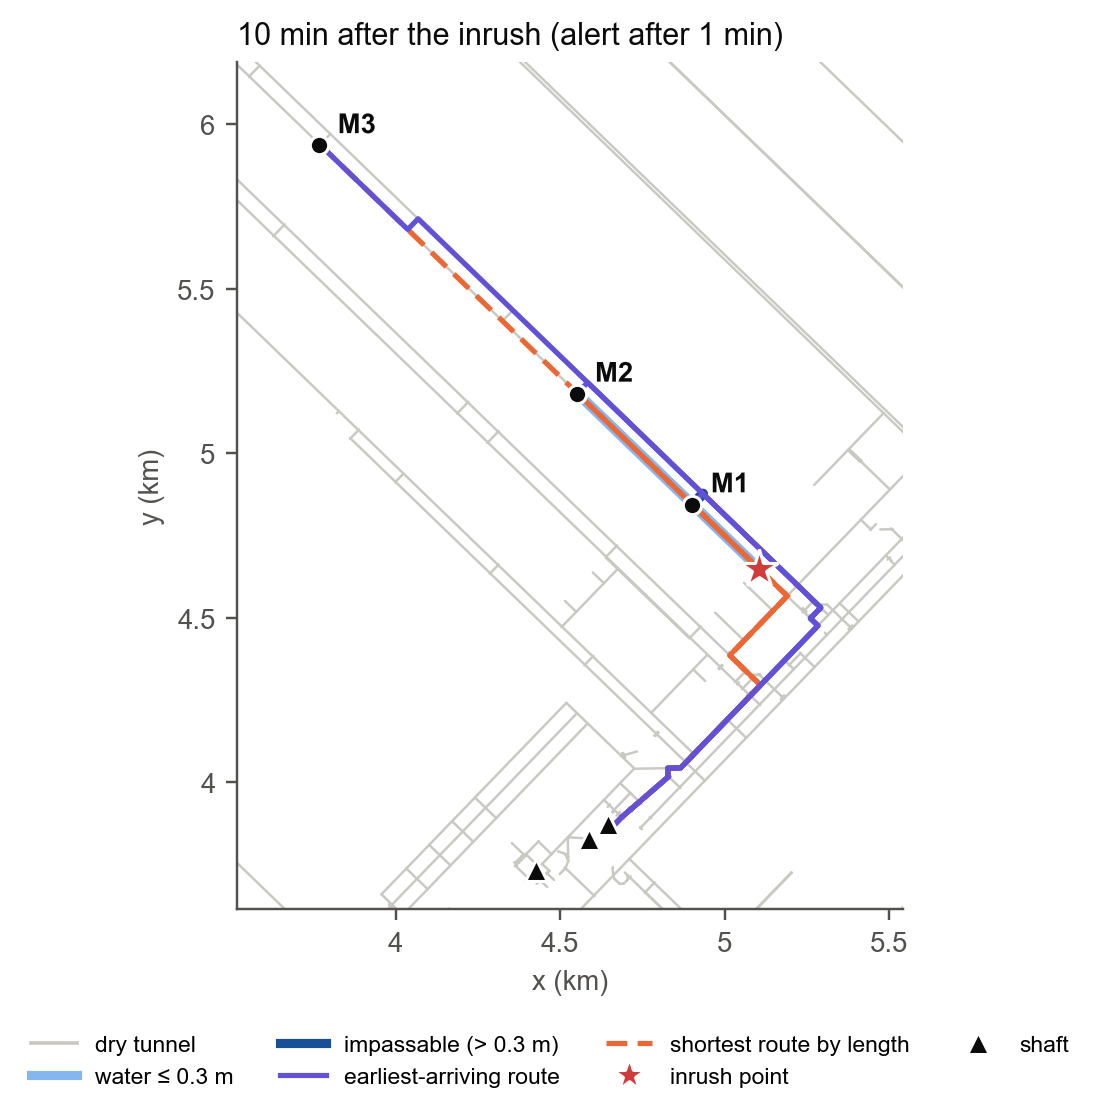
\includegraphics[width=0.62\textwidth]{figures/mine_flood_routes.png}
  \caption{Faces M1--M3 ten minutes after the onset (alert after 1 minute). The shortest routes by length (dashed) follow the roadway into which the water is spreading; the earliest-arriving routes (solid) use the parallel roadway.}
  \label{fig:mine-routes}
\end{figure}

\begin{table}[htbp]
  \centering\small
  \begin{tabular}{@{}c c c c c@{}}
    \toprule
    Face & Distance from & Earliest arrival & Shortest route & Latest alert \\
         & source (km)   & (min)            & by length (min) & $D^*$ \\
    \midrule
    M1 & 0.28 & 7.4  & 10.5      & 4.7 min \\
    M2 & 0.77 & 9.4  & 12.6      & 8.2 h \\
    M3 & 1.86 & 14.0 & 23.2      & 2.0 d \\
    M4 & 4.27 & 15.0 & identical & 13.1 d \\
    \bottomrule
  \end{tabular}
  \caption{Escape from four representative faces of the mine network, alert after 1 minute; times from the onset of the inrush.}
  \label{tab:mine}
\end{table}

\begin{table}[htbp]
  \centering\small
  \begin{tabular}{@{}c cc cc cc@{}}
    \toprule
    Alert & \multicolumn{2}{c}{M1} & \multicolumn{2}{c}{M2} & \multicolumn{2}{c}{M3} \\
    \cmidrule(lr){2-3}\cmidrule(lr){4-5}\cmidrule(l){6-7}
    (min) & earliest & shortest & earliest & shortest & earliest & shortest \\
    \midrule
    1  & 7.4 & 10.5 & 9.4  & 12.6 & 14.0 & 23.2 \\
    3  & 9.4 & 12.5 & 11.4 & 15.5 & 16.0 & 25.2 \\
    5  & --- & ---  & 13.4 & 22.6 & 18.0 & 27.2 \\
    10 & --- & ---  & 18.4 & 27.6 & 23.0 & 32.2 \\
    \bottomrule
  \end{tabular}
  \caption{Arrival times (min) of the earliest-arriving route and of the shortest route by length for different alert times. ---: no route reaches an exit.}
  \label{tab:mine-alert}
\end{table}


The shortest routes from M1--M3 follow the roadway into which the water spreads, where the miners would walk at 1--2\,m/s; the earliest-arriving routes use the parallel roadway and arrive 3.1--9.2 minutes earlier (Figure~\ref{fig:mine-routes}). Face M1 lies 0.28\,km from the source and 3\,m below it. Unless the miners there start within 4 minutes 40 seconds, no route reaches an exit. For all other faces, the latest alert exceeds 8 hours. At this inflow the threat is thus confined to a few faces near the source, and the latest alert $D^*$ identifies them directly. The scaling of Proposition~\ref{prop:scaling} holds for all 6{,}251 recorded times, and \eqref{eq:conservation} holds to a relative error below $4\times10^{-15}$.

% =====================================================================
\section{Discussion and Limitations}\label{sec:discussion}

The flood model is phenomenological. Its division rule and fixed front depth are not derived from the equations of open-channel flow \cite{chow}, and its filling rules (R2--R4) idealize the way water ponds and overtops. In particular, the depth is assumed uniform along each tunnel, whereas an inclined tunnel fills from its lower end. As Section~\ref{sec:benchmarks} shows, the forecast also depends on how tunnels are discretized: it is insensitive for most junctions but can change substantially at a few. The model has not been validated against observed inrushes or against a hydraulic solver such as SWMM \cite{swmm}; such a comparison is the most important next step.

The routing results do not depend on these specifics. Lemma~\ref{lem:fifo}, Theorem~\ref{thm:dijkstra} and Corollary~\ref{cor:latest} require only that every tunnel has a wetting time and a blocking time after which it stays impassable. They therefore apply unchanged to forecasts from any flood model in which water levels do not decrease. The routes, however, assume that the forecast is correct and known in advance. Routing for miners who observe only nearby tunnels, routing that is robust to forecast errors, and the effects of congestion and group behaviour \cite{hamacher, lu} are not considered.

The case study inherits further approximations from the data: tunnel connectivity was derived automatically and checked visually, seals and doors recorded on the plan were not modelled, elevations were interpolated between survey stations, and the tunnel height was assumed.

% =====================================================================
\section{Conclusion}\label{sec:conclusion}

We have presented a volume-conserving, event-driven flood model for tunnel networks and an exact time-dependent routing model built on its forecast. Conservation determines the filling time of a network exactly, and the monotonicity of water levels makes escape routing a FIFO problem. Dijkstra's algorithm is therefore exact, waiting is never beneficial, and the latest feasible start --- the latest alert that still leaves a way out --- is well defined and computable. On benchmark networks, the method computes routes and revised routes after a second inrush in milliseconds once the forecast is available. On a network extracted from a working mine, it shows that the danger of a moderate inrush is concentrated in a few faces near the source, and it quantifies how quickly those faces must be alerted. Coupling the routing layer to a hydraulically validated flood model is the main direction for future work.

\paragraph{Data and code availability.} The benchmark networks are those of \cite{cumcm}. The implementation, tests and the anonymized mine network are available at [repository URL].

\begin{thebibliography}{99}
\setlength{\itemsep}{2pt}\small
\bibitem{chow} V.~T. Chow. \emph{Open-Channel Hydraulics}. McGraw-Hill, New York, 1959.
\bibitem{cooke} K.~L. Cooke and E.~Halsey. The shortest route through a network with time-dependent internodal transit times. \emph{Journal of Mathematical Analysis and Applications}, 14(3):493--498, 1966.
\bibitem{cumcm} China Society for Industrial and Applied Mathematics. China Undergraduate Mathematical Contest in Modeling 2025, Problem~D: Model of water-inrush spreading and escape plans in mines, 2025.
\bibitem{cunge} J.~A. Cunge, F.~M. Holly and A.~Verwey. \emph{Practical Aspects of Computational River Hydraulics}. Pitman, London, 1980.
\bibitem{dijkstra} E.~W. Dijkstra. A note on two problems in connexion with graphs. \emph{Numerische Mathematik}, 1:269--271, 1959.
\bibitem{dreyfus} S.~E. Dreyfus. An appraisal of some shortest-path algorithms. \emph{Operations Research}, 17(3):395--412, 1969.
\bibitem{guo} Z.~Guo. A brief analysis of mine flooding problems. \emph{Management \& Technology of SME}, 2012(8):156--157. (In Chinese.)
\bibitem{hamacher} H.~W. Hamacher and S.~A. Tjandra. Mathematical modelling of evacuation problems: a state of the art. In M.~Schreckenberg and S.~D. Sharma (eds.), \emph{Pedestrian and Evacuation Dynamics}, pp.~227--266. Springer, Berlin, 2002.
\bibitem{kaufman} D.~E. Kaufman and R.~L. Smith. Fastest paths in time-dependent networks for intelligent vehicle-highway systems application. \emph{IVHS Journal}, 1(1):1--11, 1993.
\bibitem{libredwg} GNU LibreDWG, version 0.14. \url{https://www.gnu.org/software/libredwg/}.
\bibitem{lu} Q.~Lu, B.~George and S.~Shekhar. Capacity constrained routing algorithms for evacuation planning: a summary of results. In \emph{Advances in Spatial and Temporal Databases (SSTD 2005)}, LNCS 3633, pp.~291--307. Springer, 2005.
\bibitem{orda} A.~Orda and R.~Rom. Shortest-path and minimum-delay algorithms in networks with time-dependent edge-length. \emph{Journal of the ACM}, 37(3):607--625, 1990.
\bibitem{swmm} L.~A. Rossman. \emph{Storm Water Management Model User's Manual, Version 5.1}. EPA/600/R-14/413b, U.S. Environmental Protection Agency, 2015.
\end{thebibliography}

% =====================================================================
\appendix
\section{Benchmark Scenario}\label{app:coords}

\begin{table}[htbp]
  \centering\small
  \begin{tabular}{@{}l c c@{}}
    \toprule
    Point & N1 $(x, y, z)$ in m & N2 $(x, y, z)$ in m \\
    \midrule
    Source A ($s = 0$)   & (5349.03, 4931.90, 10.00) & (4143.12, 4376.28, 6.33) \\
    Source B             & (3760.40, 3808.33, 10.00), $s = 240$\,s & (5883.14, 5643.35, 40.37), $s = 300$\,s \\
    Exit E1              & (3252.16, 3326.63, 10.00) & (6336.99, 6073.22, 36.15) \\
    Exit E2              & (3173.10, 2819.97, 10.00) & (6416.05, 6579.88, 8.69) \\
    Miner M1             & (5808.18, 5367.75, 10.00) & (4395.15, 4614.53, 6.59) \\
    Miner M2             & (5194.00, 4785.31, 10.00) & (3398.34, 5965.56, 1.31) \\
    Miner M3             & (6190.81, 3434.29, 10.00) & (3879.44, 4125.47, 6.22) \\
    \bottomrule
  \end{tabular}
  \caption{Sources, exits and miners of the benchmark scenarios.}
  \label{tab:coords}
\end{table}

\end{document}
